%!TEX root = ../main.tex

In this section, we utilize the string constraint in Equation~(\ref{eqn-running}) to illustrate the approach in our work.

At first, we construct a CEFA for the regular expression $(\Sigma \setminus a)^{\{1, 60\}} (\Sigma \setminus b)^{\{1, 60\}} (\Sigma \setminus c)^{\{0, 60\}}$. Three registers are introduced, say $r_1, r_2, r_3$, to represent the three counting operators;  
the nondeterministic finite automaton (NFA) for $(\Sigma \setminus a)^* (\Sigma \setminus b)^* (\Sigma \setminus c)^*$ is constructed; the updates of registers are added to the transitions of the NFA; the counting bounds are specified by the accepting condition $1 \le r_1 \le 60 \wedge 1 \le r_2 \le 60 \wedge 0 \le r_3 \le 60$, resulting in a CEFA $\aut_1$ illustrated in Figure~\ref{fig:overview}(a). $r_1++$ means that we increment the value of $r_1$ by one after running the transition.
A string $w$ is accepted by $\aut_1$ if, when reading the characters in $w$, $\aut_1$ applies the transitions to update the state and the values of registers, reaching a final state $q$ in the end, and the resulting values of the three registers, say $v_1,v_2,v_3$, satisfy the accepting condition. In addition, we construct other two CEFAs $\aut_2$ for $\Sigma^* c^+$ (see Figure~\ref{fig:overview}(b)) and $\aut_3$ for string length function (see Figure~\ref{fig:overview}(c)). In $\aut_3$, a register $r_4$ is used to denote the length of strings and the accepting condition is $\ltrue$ (See Section~\ref{subsec:regex2cefa} for more details about the construction of CEFA.) Note that we represent the counting operators symbolically by registers instead of unfolding them explicitly. 


\begin{figure}[ht]
\vspace{-3mm}
  \centering
  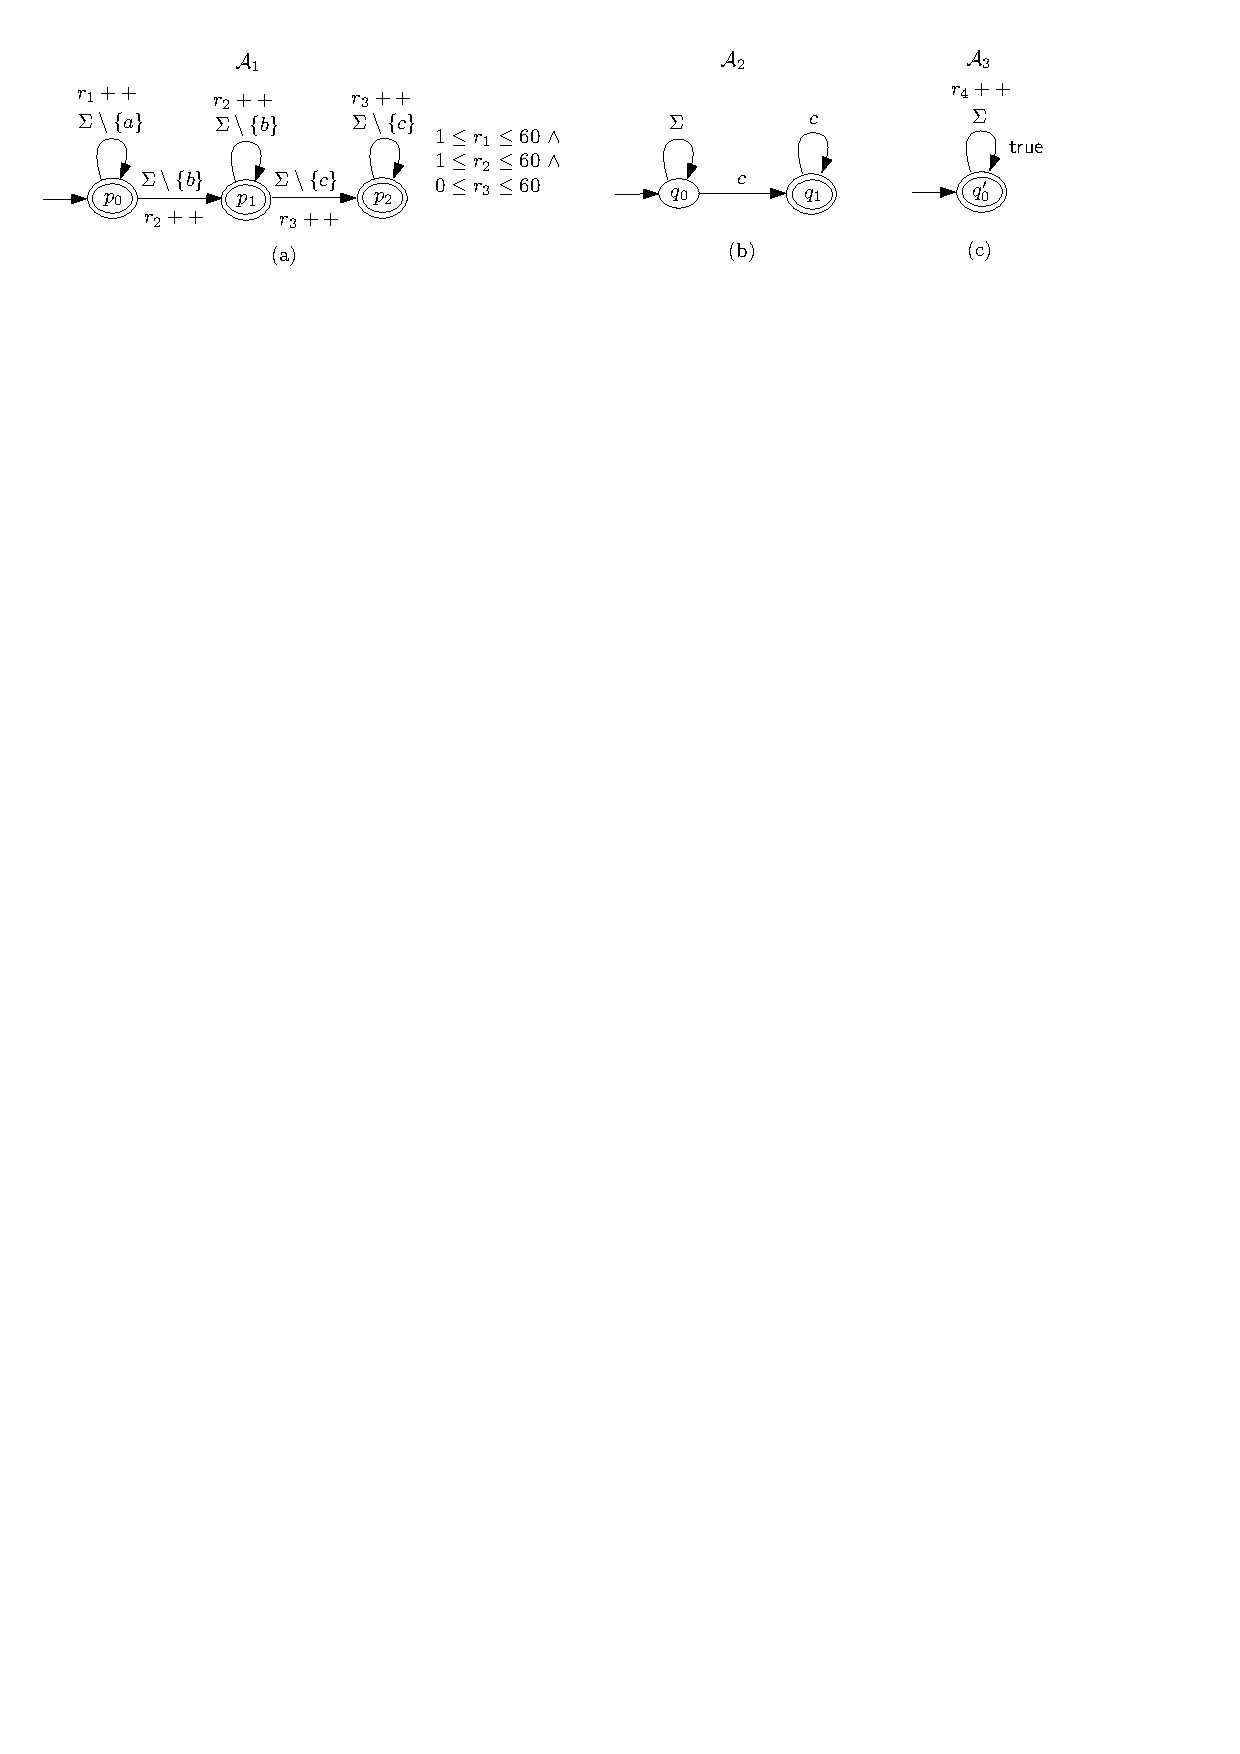
\includegraphics[width = 0.9\textwidth]{sections/overview-cefa.pdf}
  \caption{CEFA for $(\Sigma \setminus a)^{\{1, 60\}} (\Sigma \setminus b)^{\{1, 60\}} (\Sigma \setminus c)^{\{0, 60\}}$, $\Sigma^* c^+$, and $|x|$}
  \label{fig:overview}
\vspace{-3mm}
\end{figure}

Next, 
we construct $\aut_1 \cap \aut_2 \cap \aut_3$, that is, the intersection (aka product) of $\aut_1$, $\aut_2$, and $\aut_3$, as illustrated in Figure~\ref{fig:overview:product}(a), where the states can not reach the final states are removed. 
For technical convenience, we also think of the updates of registers in transitions as vectors $(u_1, u_2, u_3, u_4)$, where $u_i \in \Int$ is the update on the register $r_{i}$ for each $i \in [4]$. For instance, the transitions corresponding to the self-loop around $(p_0, q_0, q'_0)$ are thought as $((p_0, q_0, q'_0), a', (p_0, q_0, q'_0), (1,0,0,1))$ with $a' \in \Sigma \setminus \{a\}$, since $r_1$ and $r_4$ are incremented by one in these transitions. After considering the updates of registers as vectors, the CEFA is like Figure~\ref{fig:overview:product}(b).

\begin{figure}[ht]
\vspace{-4mm}
  \centering
  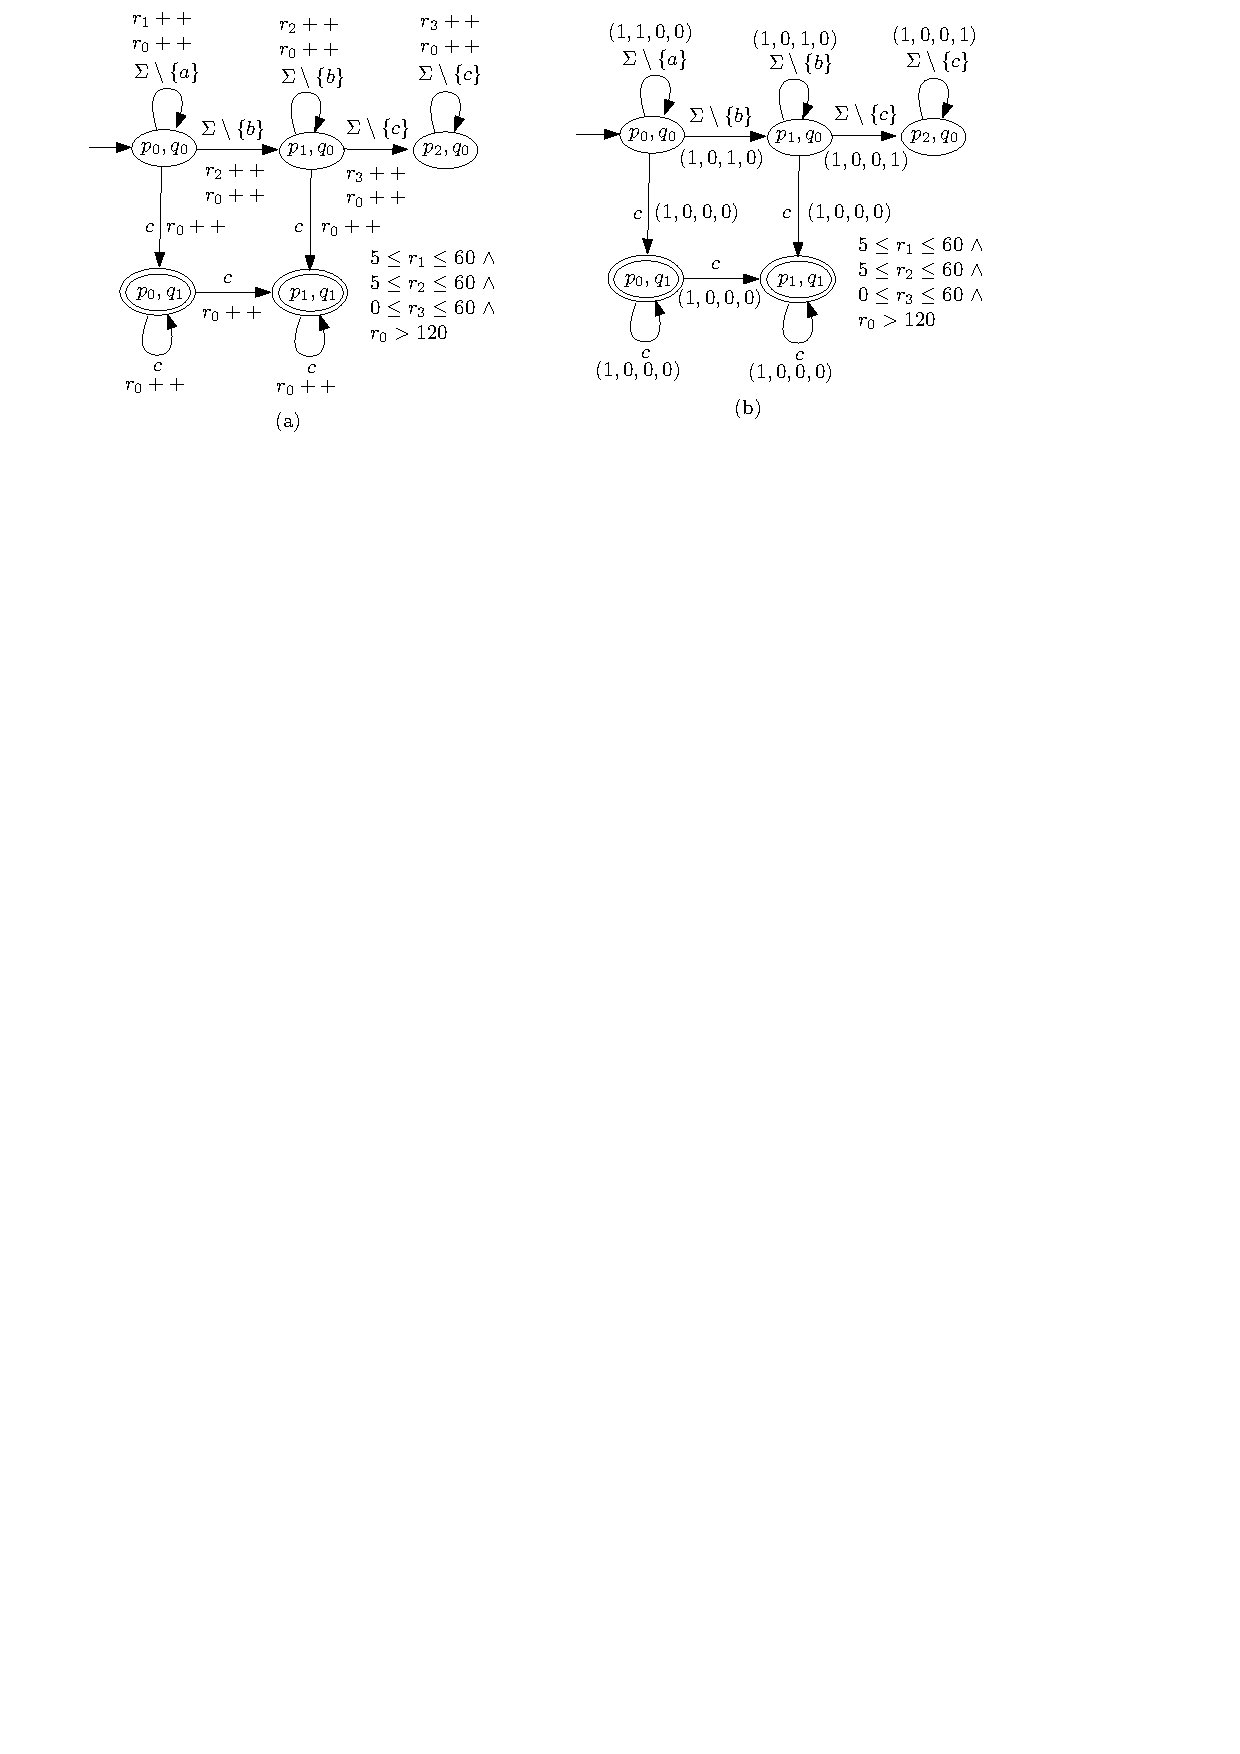
\includegraphics[width = 0.9\textwidth]{sections/overview-cefa-product.pdf}
  \caption{$\aut_1 \cap \aut_2 \cap \aut_3$: Intersection of $\aut_1$, $\aut_2$, and $\aut_3$}
  \label{fig:overview:product}
\vspace{-4mm}
\end{figure}

Finally, the satisfiability of the original string constraint is reduced to the nonemptiness of the CEFA $\aut\equiv \aut_1 \cap \aut_2 \cap \aut_3$ with respect to the LIA formula $\varphi \equiv r_4 > 120$, that is, whether there exist $w \in \Sigma^*$ and $(v_1, v_2, v_3, v_4) \in \Int^4$ such that $w$ is accepted by $\aut$, so that the resulting registers values $(v_1, v_2, v_3, v_4)$ satisfy both $1 \le v_1 \le 60\wedge 1 \le v_2 \le 60 \wedge 0 \le v_3 \le 60$ and $\varphi$. 
It is not hard to observe that the nonemptiness of $\aut$ with respect to $\varphi$ is independent of the characters of $\aut$.  Therefore, the characters in $\aut$ can be ignored, resulting into an NFA $\cB$ over the alphabet $\costset$, where $\costset$ is the set of vectors from $\Int^4$ occurring in the transitions of $\aut$ (see Figure~\ref{fig:overview:product:reduced}(a)). Then the original problem is reduced to the problem of deciding whether there exists a string $w' \in \costset^*$ that is accepted by $\cB$ and its Parikh image (i.e., numbers of occurrences of characters), say $\eta_{w'}: \costset \rightarrow \Nat$, satisfies $1 \le v'_1 \le 60\wedge 1 \le v'_2 \le 60 \wedge 0 \le v'_3 \le 60 \wedge v'_4 > 120$, where $(v'_1, v'_2, v'_3, v'_4) =  \sum \limits_{\myvec{v} \in \costset} \eta_{w'}(\myvec{v}) \myvec{v}$ for each $\myvec{v}\in \costset$. Intuitively, $(v'_1, v'_2, v'_3, v'_4)$ is a weighted sum of vectors $\myvec{v} \in \costset$, where the weight is the number of occurrences of $\myvec{v}$ in $w'$. (See Section~\ref{subsec:cefadec} for more detailed arguments.)

\begin{figure}[ht]
\vspace{-2mm}
  \centering
  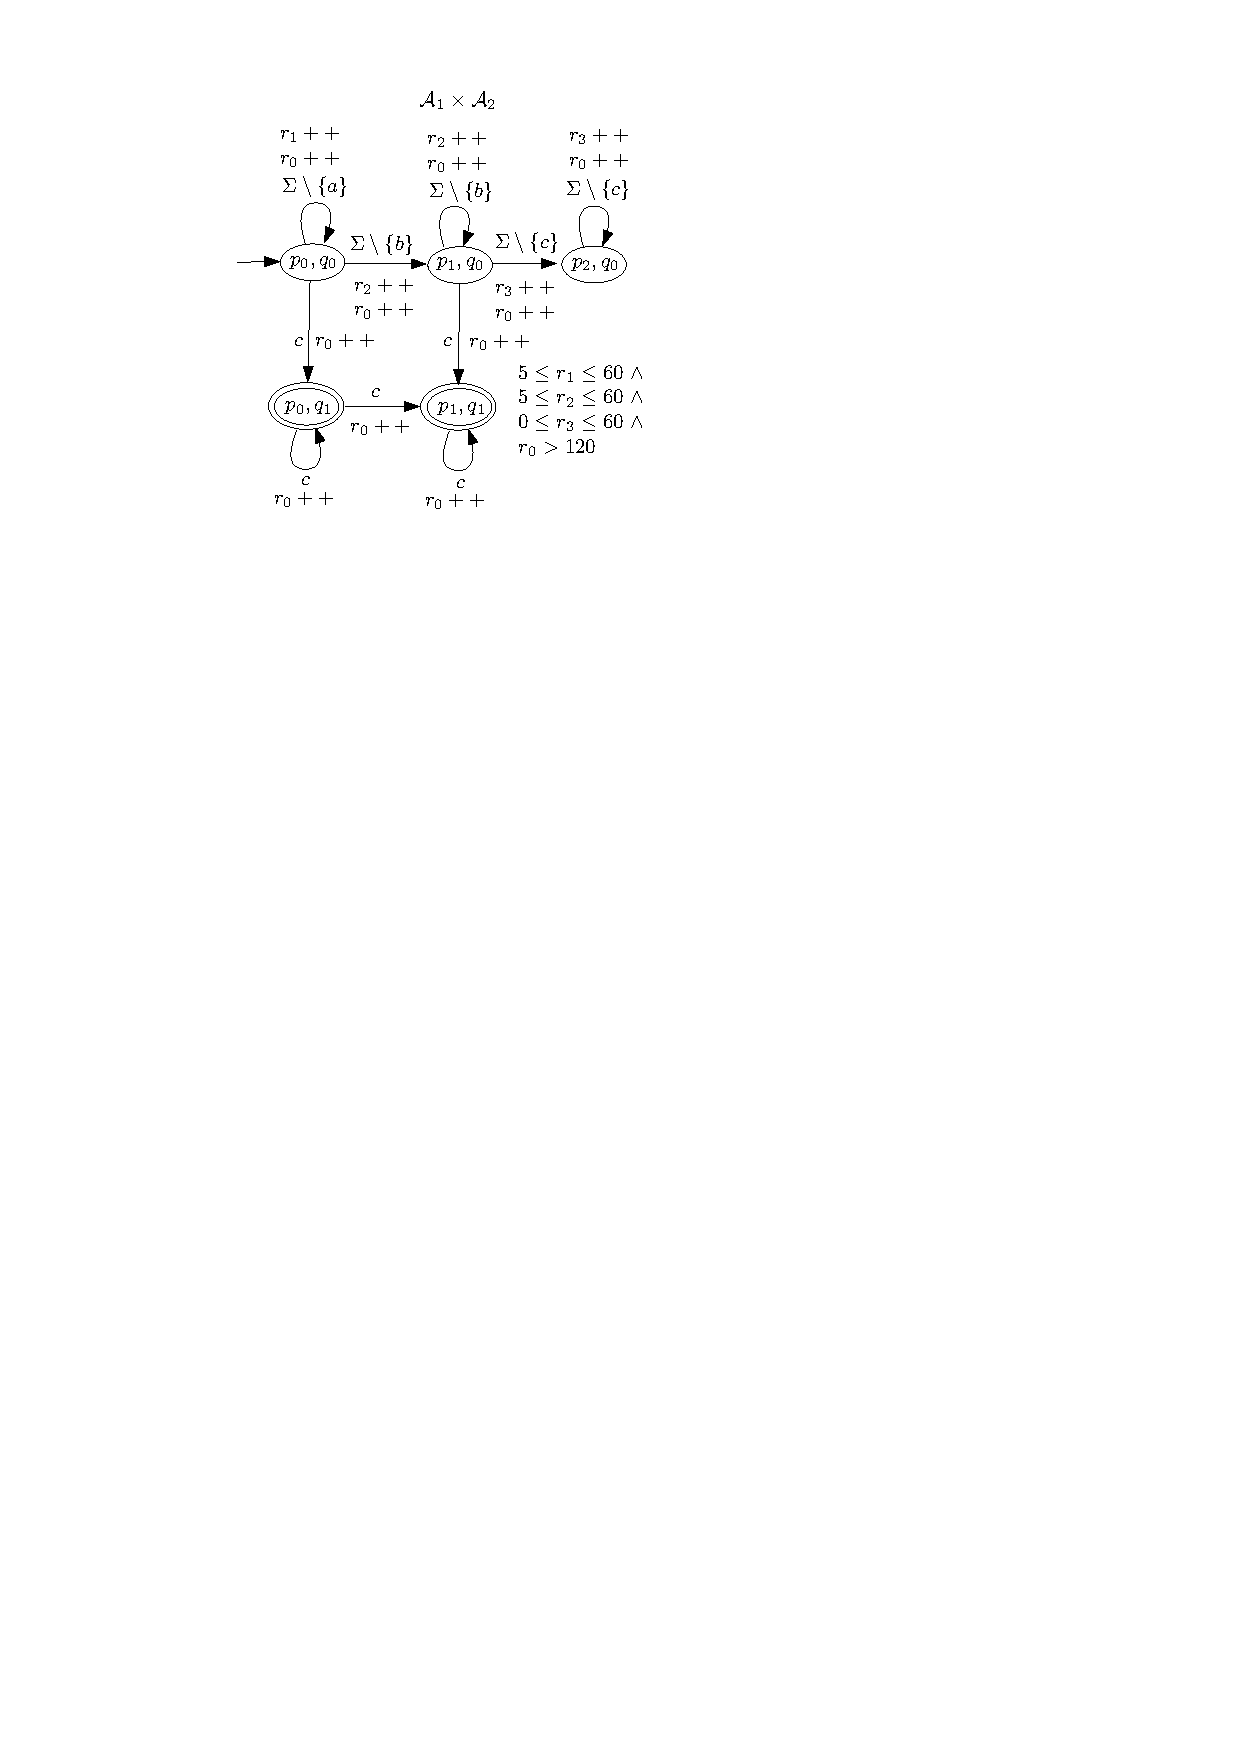
\includegraphics[width = 0.8\textwidth]{sections/overview-cefa-reduced.pdf}
  \caption{Reduced automaton $\cB$ and $\cC$}
  \label{fig:overview:product:reduced}
\vspace{-4mm}
\end{figure}
%
Let $\costset = \{\myvec{v_1}, \cdots, \myvec{v_m}\}$. 
From the results in \cite{SSMH04,VSS05}, an existential LIA formula $\psi_\cB(\anivar_1, \cdots, \anivar_m)$ can be computed to define the Parikh image of strings that are accepted by $\cB$, where $\anivar_1, \cdots, \anivar_m$ are the integer variables to denote the number of occurrences of $\myvec{v_1}, \cdots, \myvec{v_m}$.
Therefore, the satisfiability of the string constraint in~(\ref{eqn-running}) is reduced to the satisfiability of the following existential LIA formula,
\begin{equation}\label{eqn-LIA}
\begin{array}{l}
\psi_\cB(\anivar_1, \cdots, \anivar_m) \wedge \bigwedge \limits_{1 \le j \le 4} r_j = \sum \limits_{1\le k \le m}  \anivar_k v_{k, j}\ \wedge \\
1 \le r_1 \le 60 \wedge 1 \le r_2 \le 60 \wedge 0 \le r_3 \le 60 \wedge r_4 > 120.
\end{array}
\end{equation}
which can be solved by the off-the-shelf SMT solvers.

Nevertheless, when the original regexes are complicated (e.g. contain occurrences of negation or intersection operators), the sizes of the NFA $\cB$ can still be big and the sizes of the LIA formulas defining the Parikh image of $\cB$ are also big. Since the satisfiability of LIA formulas is an NP-complete problem \cite{Haase18}, big sizes of LIA formulas would be a bottleneck of the performance. 
To tackle this issue, we propose techniques to reduce the sizes of the NFA $\cB$.

Specifically, to reduce the sizes of $\cB$, we determinize $\cB$, and apply the minimization algorithm to the resulting deterministic finite automaton (DFA), resulting in a DFA $\cC$, as illustrated in Figure~\ref{fig:overview:product:reduced}(b). 
Note that $\cC$ contains only three states $q''_0, q''_1, q''_2$ and six transitions, while $\cB$ contains four states and eight transitions. Furthermore, if $\cB$ contains $\vec{0}$-labeled transitions, then we can take these transitions as $\epsilon$-transitions and potentially reduce the sizes of automata further. 

We implement all the aforementioned techniques on the top of OSTRICH, resulting in a solver $\ostrichrecl$. It turns out that $\ostrichrecl$ is able to solve the string constraint in~(\ref{eqn-running}) within one second, while the state-of-the-art string solvers are incapable of solving it within 120 seconds. 
